% Metódy inžinierskej práce

\documentclass[10pt,twocolumn,twoside,english,a4paper]{article}

\usepackage[english]{babel}
%\usepackage[T1]{fontenc}
\usepackage[IL2]{fontenc} % lepšia sadzba písmena Ľ než v T1
\usepackage[utf8]{inputenc}
\usepackage{graphicx}
\usepackage{comment}
\usepackage{amsmath}
\usepackage{url} % príkaz \url na formátovanie URL
\usepackage{hyperref} % odkazy v texte budú aktívne (pri niektorých triedach dokumentov spôsobuje posun textu)

\usepackage{cite}
%\usepackage{times}

\pagestyle{headings}

\title{Comparison of Deep Learning Algorithms in Image Recommendation Systems\thanks{Semestrálny projekt v predmete Metódy inžinierskej práce, ak. rok 2024/25, vedenie: Pavol Baťalík}} 

\author{Tomáš Kordoš\\[2pt]
	{\small Slovenská technická univerzita v Bratislave}\\
	{\small Fakulta informatiky a informačných technológií}\\
	{\small \texttt{xkordost@stuba.sk}}
	}

\date{\small 23. septembra 2024}

\begin{document}

\maketitle

\begin{abstract}
The most important currency in the world of social media is attention. The better the recommended content is, the more time people spend on the platform. Individual platforms try to improve their strategies every day. People spend hours scrolling on social media daily. That's why these applications need to develop an efficient recommendation system. In this paper I'll describe recommendation system algorithms, image classification algorithms and how a recommendation system works in general. I'll also describe real life implementations from social media technology giants such as Instagram or Twitter published on their blogs. 
\end{abstract}
\section{Introduction} \label{introduction}

Methods of recommending content include collaborative filtering \ref{applications/collaborative-filtering}, content-based filtering \ref{applications/content-based-filtering}, and machine learning algorithms.\cite{10142790} This paper tries to explain and compare convolutional neural networks \ref{nn} used to recommend images on social media.

Most large corporations remain closed-source, keeping competition on the internet. With a few exceptions, with the the recent change of X (Twitter) going open-source. 
\section{Applications} \label{applications}

Implementations of neural networks \ref{nn} (sometimes referred to as the black box) have been used for decades. The goal is to recommend visually similar images to those, which has user interacted with. Furthermore, this system can recommend advertisements which translate into revenue for the social platform. 

\begin{figure}[h]
    \centering
    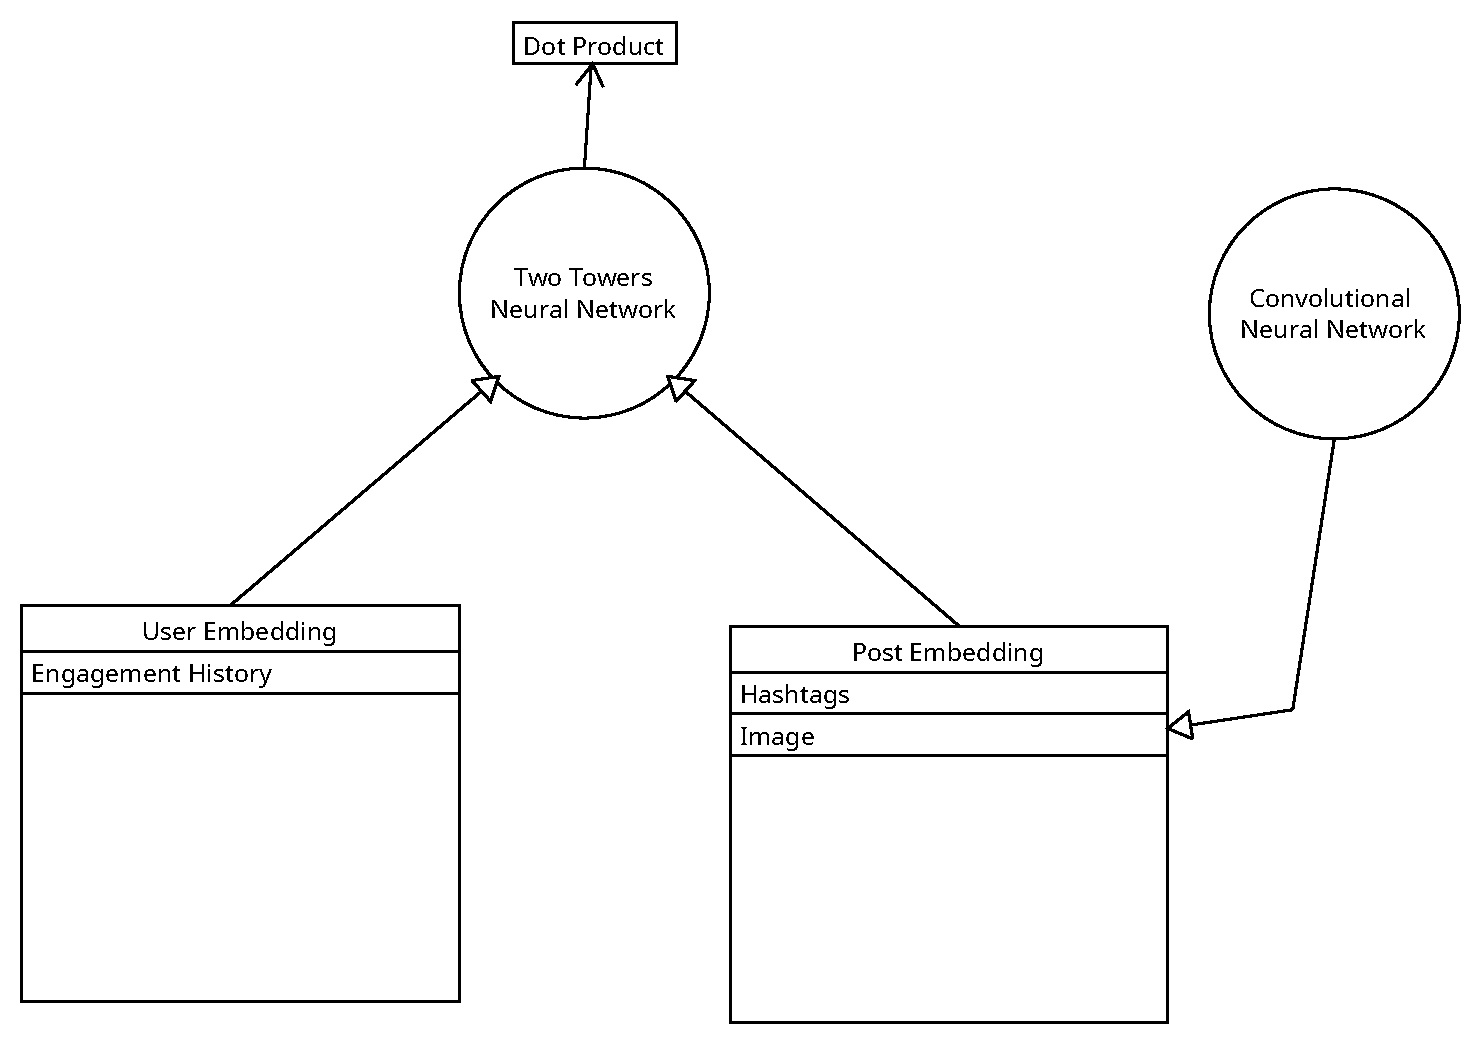
\includegraphics[width=0.7\linewidth]{Diagrams/architecture.pdf}
    \caption{Proposed architecture for content based image recommendation system}
    \label{fig:proposed-alogrithm}
\end{figure}

One of the main challenges in recommendation systems is recommending a new post to users, which hasn't been scored before. Such a problem is called ‘Cold Start' \ref{cold-start} problem. \cite{10373857} Same goes for recommending posts to a new user

\subsection{Content Based Filtering}\label{applications/content-based-filtering}

This type of filtering uses machine learning to make sure people are always seeing content that is the most interesting and relevant to them \cite{ig-new-content}


\subsection{Collaborative Filtering}\label{applications/collaborative-filtering}

To compare similarity of two accounts, this method calculates the cosine distance or dot product of two accounts. \cite{ig-explore} This way, users are filtered into groups of people with the same interests. After you have engaged with content from accounts of a certain group, you will be recommended more content from similar accounts. 

\begin{figure}[h]
    \centering
    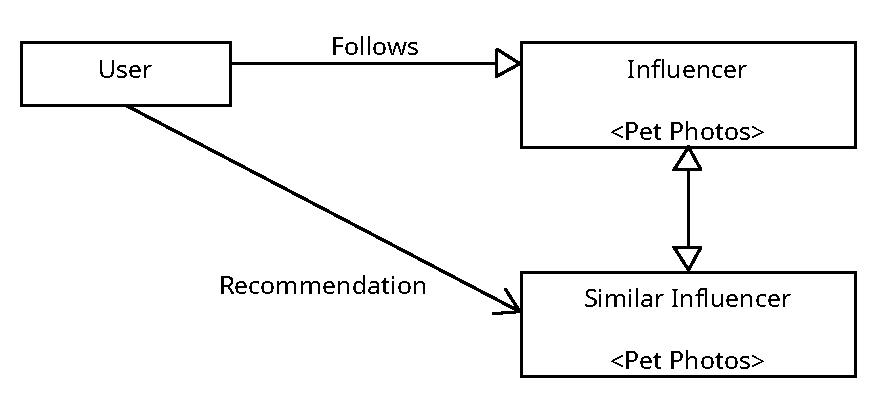
\includegraphics[width=0.7\linewidth]{Diagrams/collaborative-filtering.pdf}
    \caption{Example of account recommendation}
    \label{fig:collaborative-filtering-diagram}
\end{figure}
\section{Two Tower Neural Networks} \label{nn}
A typical Neural Network takes in two inputs, In a two towers neural network used in social media recommendation system, one is an user object and another one is a post object.

\begin{figure}[H]
    \centering
    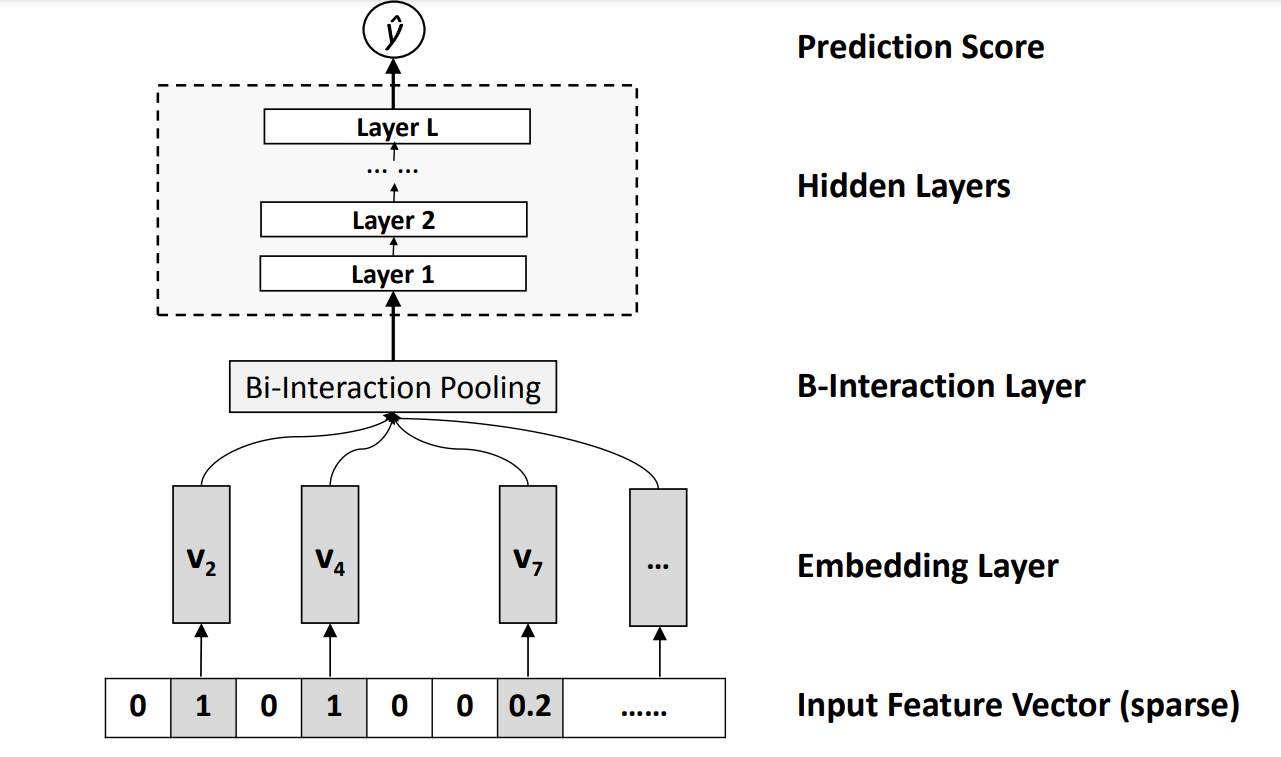
\includegraphics[width=1\linewidth]{Images/single-tower.png}
    \caption{Tower in Two Towers Neural Network \cite{10.1145/3038912.3052569}}
    \label{fig:collaborative-filtering-diagram}
\end{figure}

Above the input layer is the embedding layer; it is a fully
connected layer that projects the sparse representation to
a dense vector.  \cite{10.1145/3038912.3052569} \cite{DBLP:journals/corr/abs-1708-05027} To calculate the output of each tower, we use a neural network. A dot or cosine product is then calculated from the outputs of both neural networks.

\begin{figure}[H]
    \centering
    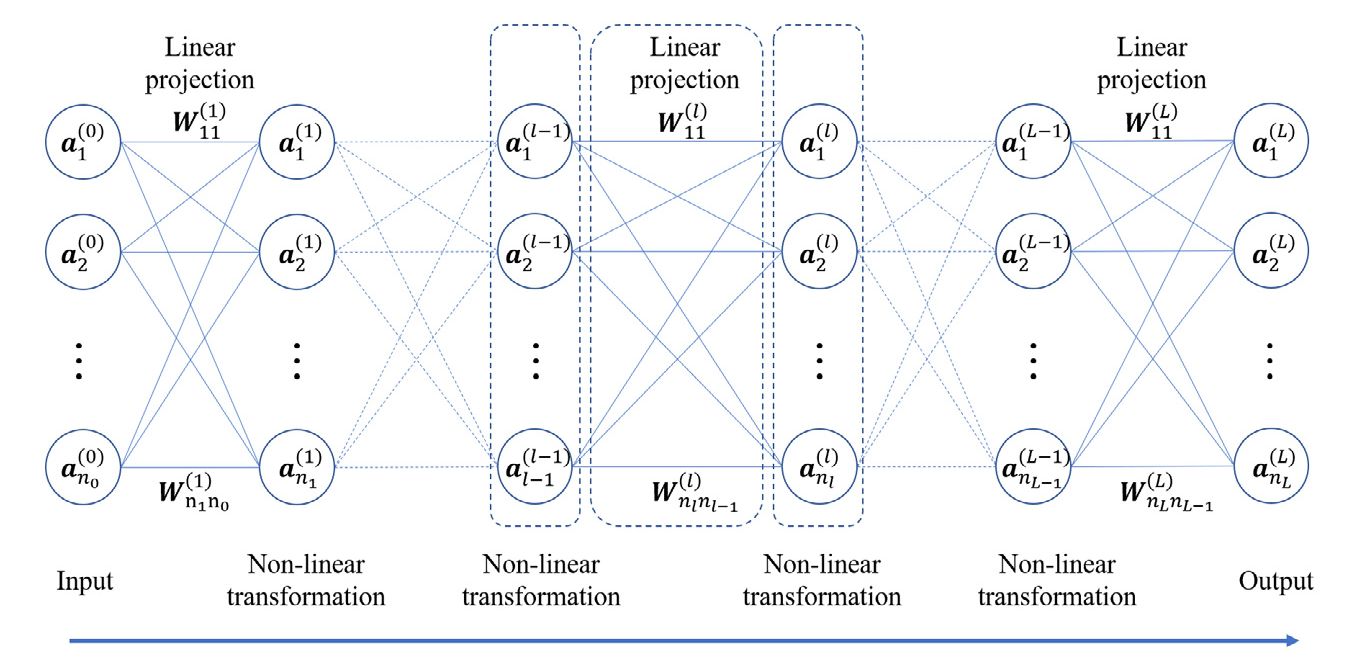
\includegraphics[width=1\linewidth]{Images/neural-network.png}
    \caption{Hidden Layers in A Typical Neural Network \cite{GAO2020409}}
    \label{fig:collaborative-filtering-diagram}
\end{figure}

Between the input and the output of a neural network are layers, each of the layers has a certain amount of neurons. \cite{GAO2020409} The value of the output is calculated from adding weighted values of the previous layer. The same applies for every node of hidden layers. The value of a node $y$ can be calculated with following formula. \cite{9784987} 

\[ y = b + \sum_{i=1}^{n} x_i w_i  \]\

Where $x_i$ is a value previous node and $w_i$ weight associated with it. We calculate sum of weighted values from every single node from previous layer. In the training process some nodes weights will become zero, therefore some nodes can be switched off. Additionally we can introduce a bias $b$ to reduce the error, because it's not affected by the weights. 

\begin{comment}
    $\begin{bmatrix}
    1 & 2 & 3\\
    a & b & c
    \end{bmatrix} $ is a matrix
\end{comment}

\subsection{Embedding}

\subsection{Cold Start}\label{cold-start}

When a new user registers on a social platform, the platform doesn't have any history about the user. Hence, it cannot personalize user's timeline. One option could be to initialize the user vector randomly, or find a similar vector to the most popular ones.

An option for creating embeddings of new posts would be analyzing the content features like the photo, description and hastags.

To improve the precision of recommendation of new items, here are a few proposed algorithms. 

\begin{comment}

aTwo tower neural network architecture 
User embedding
Post embedding
embedding = vector
normalize vector
dot product of post and user vector
pre trained embeddings

\end{comment}

\section{Convolutional Neural Networks}\label{cnn}
Basic Neural Network Concepts apply. \ref{nn} Instead of an input vector, now we have a matrix (an image). Similarly to an elemental neural network, picking a small segment from the input layer, called a filter, creates a point in the next layer. \cite{8609672} This layer is now used as an input for the next layer.

\begin{figure}[H]
    \centering
    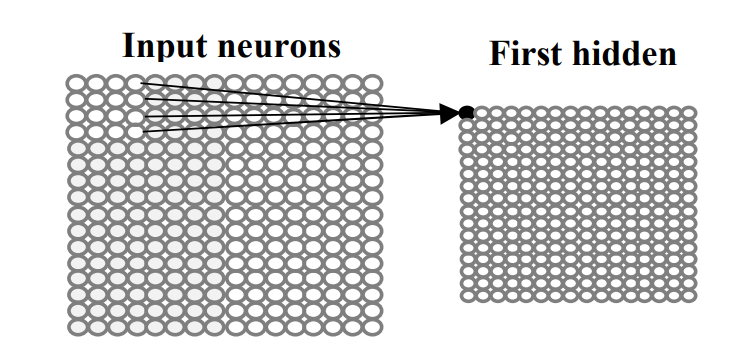
\includegraphics[width=0.5\linewidth]{Images/cnn-layer.png}
    \caption{Basic CNN model with one layer \cite{8609672}}
    \label{fig:collaborative-filtering-diagram}
\end{figure}

The difference between one dimensional neural networks and 2D matrix neural networks is that we can visualise each layer or kernel as an image. Thus we can understand simple convolutional networks better. Some layers are perceived as 3D because of the color depth available.

\begin{figure}[H]
    \centering
    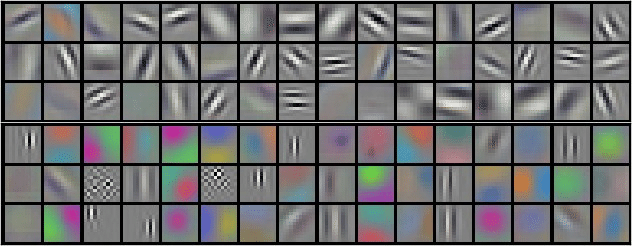
\includegraphics[width=0.5\linewidth]{Images/kernels.png}
    \caption{Kernels learned from AlexNet's first convolutional layer.   \cite{shehata2016using}}
    \label{fig:collaborative-filtering-diagram}
\end{figure}

The final output layer is a vector with probabilities, every value represents propability of the image being classified in a specific class (eg. cat, dog, bird, etc.)



\begin{comment}
\subsection{Alex Net}

\url{https://github.com/amir-saniyan/AlexNet}

\url{https://proceedings.neurips.cc/paper_files/paper/2012/file/c399862d3b9d6b76c8436e924a68c45b-Paper.pdf}

\subsection{VGGNet}

\url{https://github.com/deepblacksky/VGG_tensorflow?tab=readme-ov-file} 

\url{https://arxiv.org/abs/1409.1556}
\subsection{ResNet}

\subsection{GoogLeNet}
GoogLeNet (Inception)

\url{https://github.com/conan7882/GoogLeNet-Inception}

\url{https://research.google/pubs/going-deeper-with-convolutions/}
\subsection{EfficientNet}

\url{https://arxiv.org/abs/1905.11946}

\url{https://github.com/qubvel/efficientnet}
\subsection{Siamese Networks}

\url{https://www.cs.cmu.edu/~rsalakhu/papers/oneshot1.pdf}

\subsection{X (Twitter)}\label{cnn/xalgorithm}

\url{https://github.com/twitter/the-algorithm}

\url{https://blog.x.com/engineering/en_us/topics/open-source/2023/twitter-recommendation-algorithm}

RAPID NET

\end{comment}
\section{Future Use} \label{future}
\section{Conclusion} \label{conclusion} 


\bibliography{literatura}
\bibliographystyle{abbrv} % prípadne alpha, abbrv alebo hociktorý iný
\end{document}
